\graphicspath{{../images/ch3/}}	% Image directory


\chapter{Resistive pulse studies of aspherical mesoparticles}
\label{chap:rods}
	

	\section{Background \& Theory}
		In the introduction of this dissertation we introduced and explained the theory behind resistive pulse sensing, a particle characterization technique that works by monitoring the change in conductance of a nanopore as small particles pass through it. Probably the most important application of RP sensing is in measuring the sizes of particles. An analytic model was devised by DeBlois \emph{et al.} to relate the size of a particle to its resistive pulse amplitude. The solution is essentially an electrostatics boundary-value problem: given an insulating particle inside a pore and a known externally applied voltage, calculate the electric field distribution inside the pore, and from the electric field distribution calculate the pore's expected resistance with the particle inside it. When this calculation is performed for spherical particles travelling along the axis of long cylindrical pores, the change in resistance or current is found to be
		
		\begin{equation}\label{eq:dI}
			\frac{\Delta R}{R_{0}}=\frac{\Delta I}{I_{p}}=\frac{3}{2}\left[1-0.8\left(\frac{d}{D}\right)^{3}\right]\frac{v}{V}.
		\end{equation}
		
		
		

		
		
		
		Equation \ref{eq:dI} is useful for relating the change in current---or resistance---to the diameter of spherical particles. The factor of $\frac{v}{V}$ is no accident---it reflects that the primary reason for the change in resistance of the channel is from the loss of conductive volume in the pore due to the presence of the insulating particle. 
		
		\begin{figure}[t!]
			\centering
			\begin{subfigure}[t]{0.5\textwidth}
				\centering
				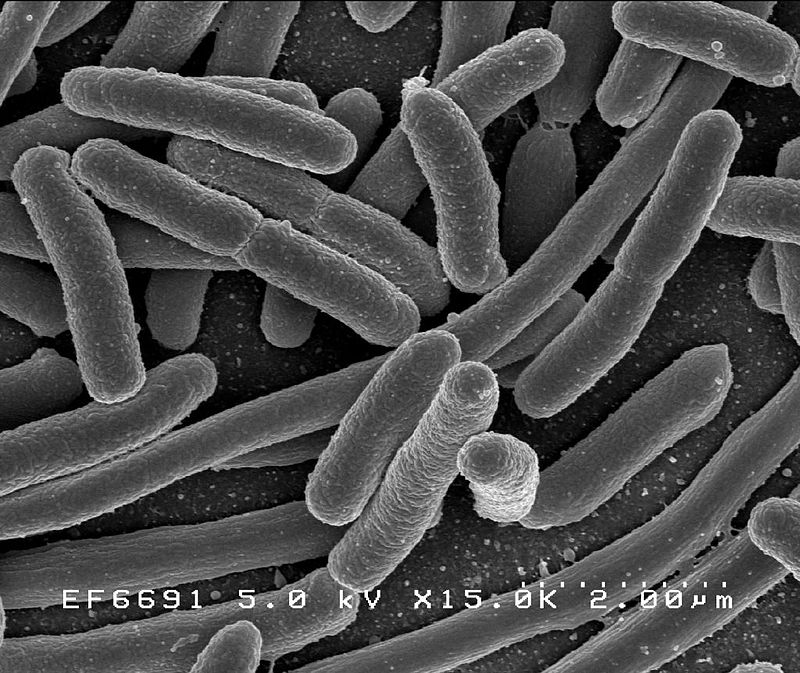
\includegraphics[width=2in]{ecoli.jpg}
				\caption{Escherichia coli (E. coli) bacteria.}
			\end{subfigure}
			\begin{subfigure}[t]{0.5\textwidth}
				\centering
				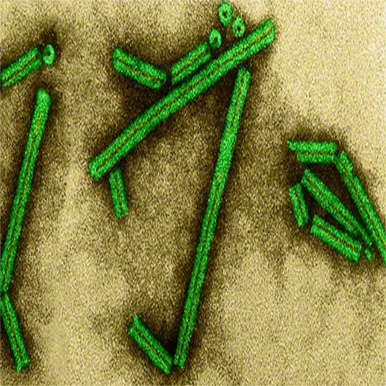
\includegraphics[width=2in]{tobaccomosaicvirus.png}
				\caption{Tobacco mosaic virus}
			\end{subfigure}
			\caption{\textbf{Two examples of natural aspherical biological entities.}}
		\end{figure}
		
		While this equation is useful, it is very often the case that particles of interest are not spherical. For instance, many biomolecules such as viruses and proteins are poorly approximated as spheres, and are more rod-like in shape (see Fig. \ref{fig:aspherical_particles.png}). In this case, the resistive pulse amplitude of on-axis translocations through a cylindrical pore is given by 
		
		\begin{equation}\label{eq:dIellipsoid}
			\frac{\Delta R}{R_{0}}=\left[f_{\perp}+\left(f_{\parallel}-f_{\perp}\cos^{2}\alpha\right)\right]\frac{v}{V},
		\end{equation}

		where $f_{\perp}$ and $f_{\parallel}$ are so called `shape-factors', that depend on the particle's major and minor axis lengths, and $\alpha$ is the orientation of the particle with $\alpha=0$ being axially aligned. Notice that again the factor of $v/V$ shows up as it did in the Eq. \ref{eq:dI}. Figure \ref{fig:dIellipsoid} shows a plot of the relative $\Delta I/I_{p}$ for various ellipsoids of the same volume but different axial lengths.
		
		\begin{figure}
			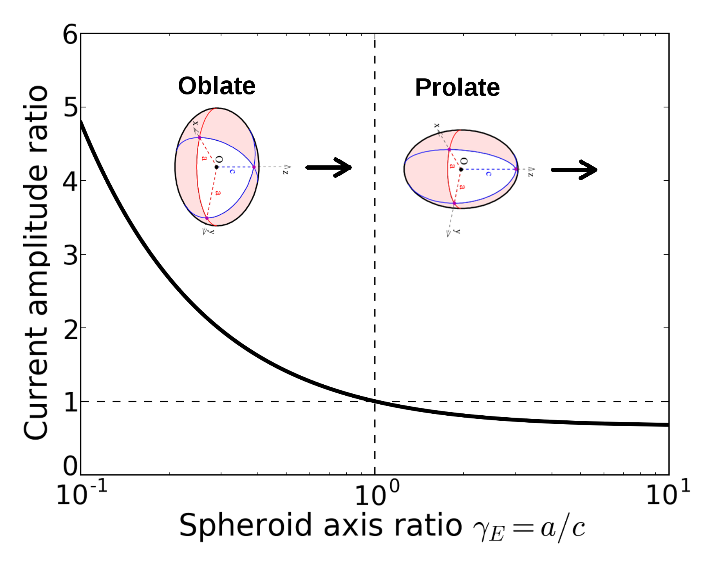
\includegraphics[width=0.5\textwidth]{dIellipsoid}
			\caption{\textbf{Resistive pulse amplitude $\Delta I/I_{p}$ relative to that of a sphere.} Inset images show the geometry of the ellipsoid. The central axis is for spheres, particles with equal axis lengths. To the right of the central line the geometry is described as prolate with respect to the direction of motion, and to the left it is oblate. The equation \ref{eq:dIellipsoid} predicts that the current amplitude decreases for prolate geometries, and sharply increases for oblate geometries.}
			\label{fig:dIellipsoid}
		\end{figure}


		
		While equation \ref{eq:dIellipsoid} is useful for determining the volume of spheroidal particles from their resistive pulse amplitudes, it would be useful to devise a method for measuring the length of particles in addition to measuring their volumes as an additional physical marker for their identification in a sample. However, it is not immediately obvious how this could be achieved. In the following sections, we suggest a measurement protocol that can be used to determine the length of particles, first in a qualitative manner that can be used to rank particles of different lengths, and then in a quantitative manner to actually measure the length of unknown particles.
		
		
		\subsection{Length measurement protocol}
		
			Consider a pore with a rough, non-uniform interior. Due to the irregular interior, the channel cross sections will have a range of resistance values; for instance, a large cavity in the channel will have a smaller resistance than a more narrow constriction. Therefore, we can consider the resistive pulse signals of particles passing through the pore to reflect the pore's interior shape. If we ignore the effects of electrostatic boundary conditions on the resistive pulse amplitude, the following yields the resistive pulse amplitude for non-constant width pores:
			
			\begin{equation} \label{eq:localdR}
				\Delta R\left(z'\right)=\frac{\rho}{\pi}\left[\int_{z=z'}^{z=z'+l_{p}}\left(\frac{1}{r^{2}_{P}\left(z\right)-s^{2}_{p}\left(z\right)}-\frac{1}{r^{2}_{P}\left(z\right)}\right)dz\right].
			\end{equation}
			
			\begin{figure}
				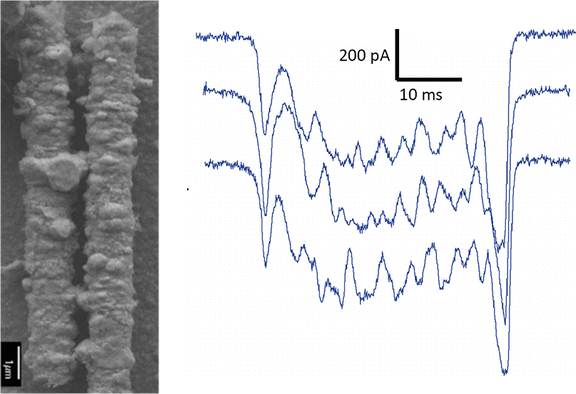
\includegraphics[width=.5\textwidth]{particlesreveal.png}
				\caption{\textbf{Metal replica of PET pores (left) and samples of resistive pulse amplitudes of polystyrene beads collected through pores of the same material (right).} The resistive pulse amplitudes is a measure of local pore resistance, and is reflective of the local pore's diameter.}
				\label{fig:particlesreveal}
			\end{figure}

			
			
			As a concrete example of when this occurs, Pevarnik \textit{et al.} performed experiments with small polystyrene beads in polyethylene terephthalate pores, and found the resistive pulse were characterized by irregular, jagged shapes. They reasoned that this non-traditional resistive pulse profile must be due to the shape of the pore itself, and confirmed the hypothesis by imaging the interiors of the pores using a reverse metal replica procedure. This concept is demonstrated in Fig. \ref{fig:particlesreveal}.
			
			
			\begin{figure}
				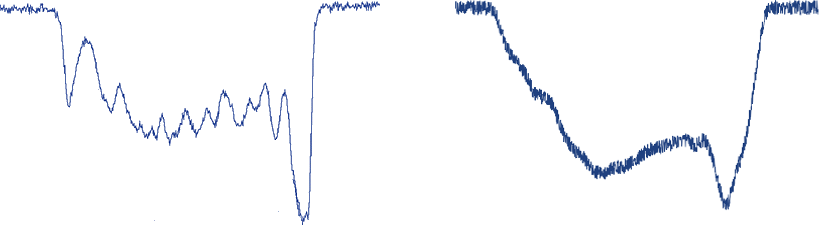
\includegraphics[width=\textwidth]{short_long_simulated.png}
				\caption{\textbf{Signal of a small sphere (left) and simulated signal of a longer particle (right) through a PET pore.} While the short particle reveals the pore's small scale interior features, the longer particle is not capable of resolving these features.}
				\label{fig:short_long_simulated}
			\end{figure}

			
			
			So far we have made mention of the \textit{local} pore radius. From Eq. \ref{eq:localdR}, we can see that the change in resistance is only due to the area of solution surrounding the particle, and does not depend on the resistance of the pore elsewhere. According to this equation, not only do pores measure the interior geometry of the pore, but they measure it with a \textit{length dependent} resolution. For particles that are shorter than the characteristic length scale fo the undulations in the channel, the resistive pulses are high resolution mappings of the inner pore geometry. These small particles are able to explore minor cavities and protrusions in teh channel. On the other hand, if we consider a particle whose length extends along many of such irregularities, it may occupy several different regions of resistance at a time. In this case, the particle maps the pore's inner geometry with a low resolution. Figure \ref{fig:short_long_simulated} shows an example of a sphere passing through a PET pore alongside a simulation of the signal a longer particle would produce. The key difference between the two is in there resolution, as described above. While the small sphere is able to reveal the fine features of the pore's interior, the longer particle's signal averages over these features.
			
			\begin{figure}
				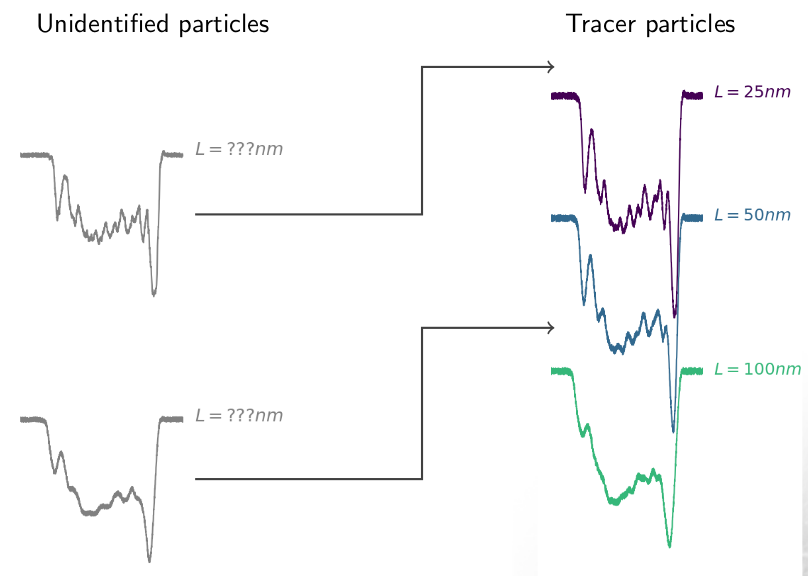
\includegraphics[width=\textwidth]{qualitative_length_measurement.png}
				\caption{\textbf{Protocol for qualitatively determining particle length.} Resistive pulse signals of particles of unknown and known length are shown on the left and right, respectively. The particles of known length on the right are `tracer particles', particles that are recorded so as to provide a means for comparing other particles' signals with. Each unknown particle is ranked according to the resolution its signal provides and compared with the tracer particles' signals. This method does not yield an accurate measure of length, but can be used to obtain a semi-quantitative estimate.}
				\label{fig:qualitative_length_measurement}
			\end{figure}
			
			The above arguments reveal that the signals of short and long particle sthrough irregular pores are fundamentally different, and this immediately suggests a means for qualitatively determining the length of a particle. First, we pass `tracer particles', particles of known length through the pore and record their resistive pulse signals. Then, we record the passage of particles of unknown lengths. After both the tracers and unknown particles are recorded, we rank the unknown particles according to the amount of resolution present in their resistive pulse signature. Figure \ref{fig:qualitative_length_measurement} shows a picture describing this qualitative algorithm for ranking particle lengths.
			
			While this qualitative length ranking algorithm is useful, it would be desirable to devise a means for \textit{quantitatively} determining the lengths of unknown particles. In order to understand how this can be done, we rewrite Eq. \ref{eq:localdR} as follows:
			
			\begin{equation} \label{eq:localdRreexpressed}
				\begin{split}
					\frac{\Delta R_{l}}{R_{0}} &= \frac{\rho}{\pi}\left[\int_{z}^{z+l_{p}}\left(\frac{1}{r^{2}_{P}\left(z'\right)-s^{2}_{p}\left(z'\right)}-\frac{1}{r^{2}_{P}\left(z'\right)}\right)dz'\right]/R_{0} \\
					&= \sum_{i=0}^{n-1}\frac{\rho}{\pi}\left[\int_{z+il_{s}}^{z+\left(i+1\right)l_{s}}\left(\frac{1}{r^{2}_{P}\left(z'\right)-s^{2}_{p}\left(z'\right)}-\frac{1}{r^{2}_{P}\left(z'\right)}\right)dz'\right]/R_{0} \\
					&= \sum_{i=0}^{n-1}\Delta R_{s}\left(z+il_{s}\right)/R_{0}.
				\end{split}
			\end{equation}
			
			In this form of the equation, we break the integral for the change in resistance of a long particle into smaller parts of equal length. Because resistance add in series, each of these small parts of the integral corresponds to the resistance of a shorter particle, and therefore we recognize that the resistive pulse amplitude of a long particle can be reexpressed as the sum of the resistive pulse amplitudes of smaller particles at various points in the channel. This suggests a new means of \textit{quantitatively} measuring particle length: we record resistive uplse amplitudes of smaller particles, and use the transformation given by Eq. \ref{eq:localdRreexpressed} to \textit{simulate} the resistive pulse signal of a particle of longer length. We generate many such simulations over a range of lengths, and then compare each of the simulated signals with the signal of the particle of unknown length. The comparison that yields the greatest similarity is declared as the true length of the unknown particle.
			
			\begin{figure}
				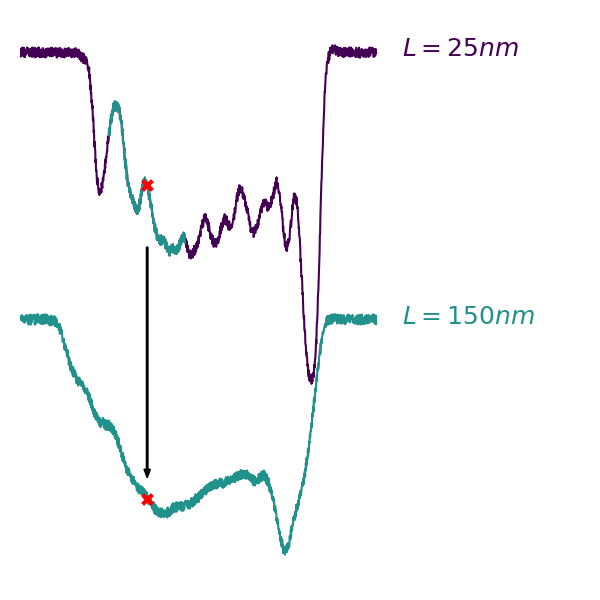
\includegraphics[width=.5\textwidth]{moving_average_process.png}
				\caption{\textbf{Visualization of the moving average process.} The teal shading in the top resistive pulse indicates the length over which the moving average is performed. This point is mapped onto a point in the transformed signal below it, and this transformation is applied to all points in the original signal.}
				\ref{fig:movingaverage}
			\end{figure}

			
			Instead of exactly using Eq. \ref{eq:localdRreexpressed}, we instead use a convolution or moving average of the signals of the shorter particles given by the following equation:
			
			\begin{equation}\label{eq:movingaverage}
				I_{i}\rightarrow I_{i}^{l'}=\frac{1}{N}\Sigma_{j=i-\frac{N}{2}}^{j=i+\frac{N}{2}}I_{j}, \mathrm{and} \\
				N=\frac{fl'}{v},
			\end{equation}
			
			where N is the total number of points in the moving average, $I_{i}$ is the $i$th current measurement in the signal of the unprocessed short particle, $I_{i}^{l'}$ is the transformed data point for a moving average over length $l'$, $f$ is the sampling frequency of the current acquisition instrument, and $v$ is the \textit{average} velocity of the particle during its translocation through the pore. However, equation \ref{eq:movingaverage} slightly oversamples particle positions in the middle of the moving average compared to particle positions at the very ends, along a distance equal to half the length of the small particle at each end. For this reason, the moving average estimate of the correct transformation should slightly overestimates the length of long particles. However, when $l\ll l'$, i.e. the tracer particle's displacement length is much less than the longer rod's displacement length, the effect is negligibly small. Figure \ref{fig:movingaverage} shows a visualization of the moving average process and its effect on the smoothed signal.

			
			After computing the moving averages of the tracer particles over an array of lengths, a similarity measure is calculated between every pair of convoluted-raw signals for the tracer particle and the long particle, and the length with the greatest similarity measure is chosen as the correct length of the particle.
			
			Probably the simplest similarity measure of two time-series is the point-wise summed Euclidean distance between the two signals given by the following formula:
			
			\begin{equation}\label{eq:euclideandistance}
				C\left(S, S'\right)=\Sigma_{i=0}^{N-1}\left(S_{i}-S'_{i}\right)^{2}.
			\end{equation}
			
			\begin{figure}
				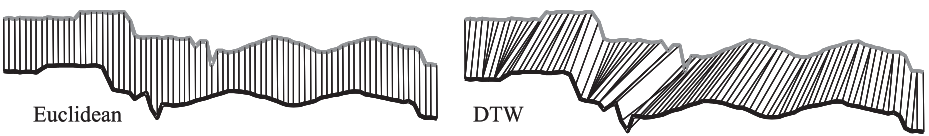
\includegraphics[width=\textwidth]{eucliddtw}
				\caption{\textbf{Comparison of standard Euclidean distance metric (left) and distance metric as determined by dynamic time warping (right).} Notice that the Euclidean distance does not take into account small displacements of the two signals in time, despite their obvious similarity. On the other hand, dynamic time warping is able to account for small mismatches in time by finding the connections between points that minimizes the total cost.}
				\label{fig:eucliddtw}
			\end{figure}

			
			However, the problem with the similarity measure in Eq. \ref{eq:euclideandistance} is it is not robust against small variations in the phases of the two signals, i.e. if the two signals evolve in time noisily in such a way that they are not instantaneously exactly in phase. For instance, Fig. \ref{fig:eucliddtw}(left) shows two resistive pulse time-series taken during an experiment and overlapped exactly in time, with lines connecting the points that would be summed in the Euclidean distance metric\cite{Keogh2005}. Notice that the two sequences are very similar, but due to a non-perfect alignment of identical features in time, the aligned Euclidean distance metric will greatly penalize the similarity of the two signals. It seems that we need a technique that is more robust against local time distortion in order to better measure the similarity of the two signals.
		
		\subsection{Dynamic time warping}
		
			One method of measuring the similarity of two time-series that accounts for time offsets is dynamic time warping. Figure \ref{fig:eucliddtw}(right) shows two time-series signals that have been aligned after dynamic time warping. The image shows that the algorithm is capable of matching points that are not perfectly aligned in time, but that reflect the actual \textit{physical} progression of the two signals. With regards to our case, local features in two RP signals that correspond to the same position in the channel may not vertically overlap perfectly in time, but the dynamic time warping algorithm is capable of recognizing that the two features are same. 
			
			\begin{figure}
				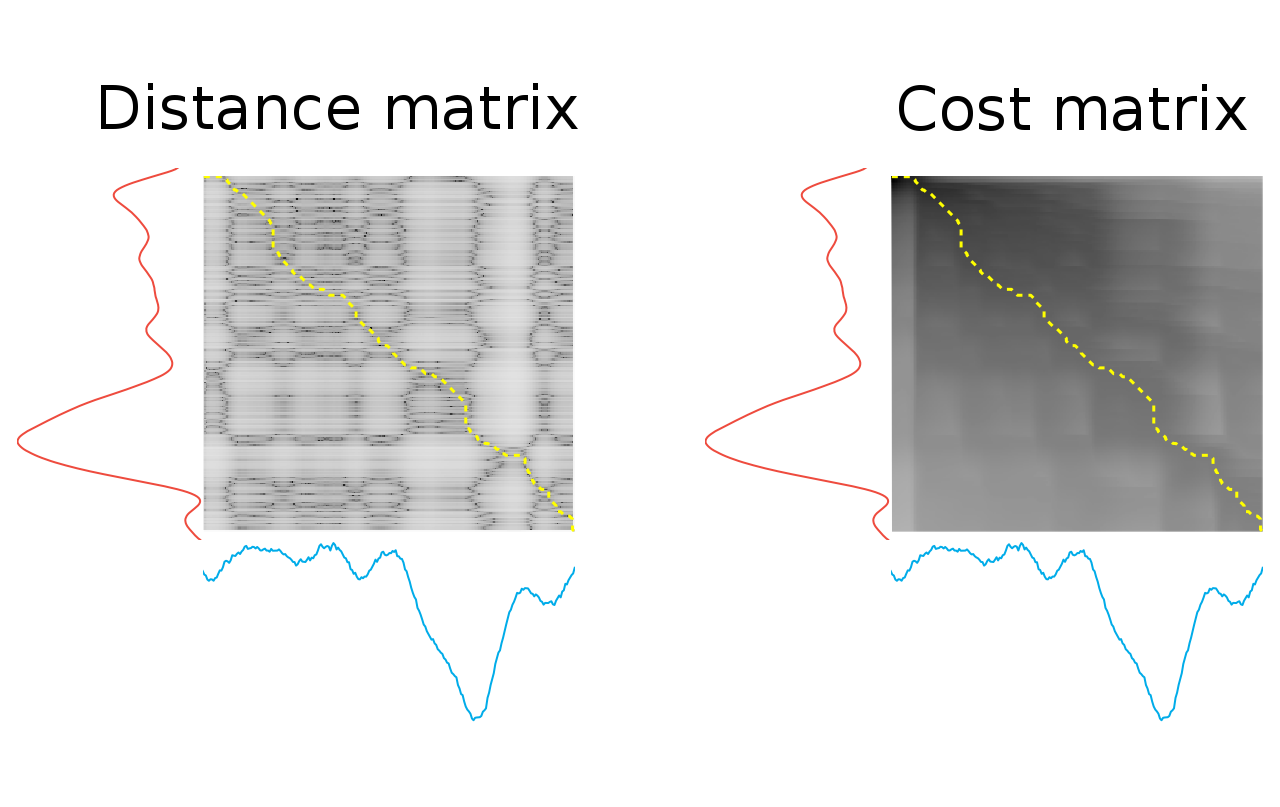
\includegraphics[width=\textwidth]{distancecost}
				\caption{\textbf{Distance (left) and cost matrices (right) of two resistive pulse signals as determined by dynamic time warping.} The element $\left(i,j\right)$ in the distance matrix represents the Euclidean distance between the two signals, $\left(S_{i}-S'_{j}\right)^{2}$. Every element in the cost matrix represents the summed Euclidean distance along the minimum path that arrives at that point. Therefore, the point at the lower right-most point in the distance matrix is the summed cost to completely connect the two signals. The path that yields the cost of that element in the matrix is represented by the yellow dashed line.}
				\label{fig:distancecost}
			\end{figure}

			
			The dynamic time warping algorithm works as follows. First, a matrix $D_{i,j}$ of the point-wise Euclidean distance between all two points in the two signals is created, as shown in Fig. \ref{fig:distancecost} (left). For instance, point $D_{3,4}$ is the Euclidean distance between point $3$ and $4$ in signals $S$ and $S'$, respectively. The objective is to traverse through the distance matrix along the path that minimizes the total accumulated distance, or the cost $C$, subject to certain kinematic constraints. Each step in the trajectory is defined by the indices from the two respective signals $\left(i,j\right)$. The non-warped Euclidean distance metric given by Eq. \ref{eq:euclideandistance} would correspond to a straight diagonal trajectory through the matrix, e.g. no warping at all. Although there are several formulations of dynamic time warping, the original method only allows for three types of motion such that $\left(i,j\right)\rightarrow\left(i+1,j\right)$ (progressive vertical motion), $\left(i,j\right)\rightarrow\left(i+1,j+1\right)$ (progressive diagonal motion), or $\left(i,j+1\right)$ (progressive horizontal motion). Regressive motion, which would correspond to taking a step backwards in the path back towards the upper left cell in the matrix, is forbidden. The key to dynamic time warping is the means by which we determine the optimal path that minimizes the total accumulated distance. The problem of finding the ideal path through the distance matrix according to the kinematic constraints is combinatorically large, and the number of unique trajectories has lower bound ${N'+N-2\choose N'-1}$, where $N, N'$ are the number of data points in each of the two signals. Due to this scaling, random searching of paths through the matrix is not a feasible means of determining the optimum path for large $N+N'$. 
			
			As the name implies, dynamic time warping (DTW) is a dynamic computational algorithm for determining the minimum path, described as follows. First, we must recognize that, due to the kinematic rules for stepping through the matrix, the minimum path to arrive at point $\left(i,j\right)$ must pass through one of points $\left(i-1,j\right)$, $\left(i-1,j-1\right)$, or $\left(i,j-1\right)$. Therefore, the cost $C$ of point $\left(i,j\right)$ is given by
			
			\begin{equation}\label{eq:dtwcost}
			C_{i,j}=D_{i,j}+\mathrm{min}\left[C_{i-1,j}, C_{i-1,j-1}, C_{i,j-1}\right].
			\end{equation}
			
			
			\begin{figure}
				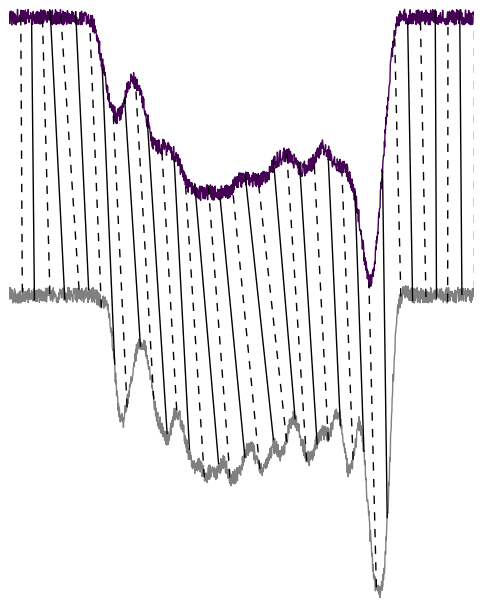
\includegraphics[width=.5\textwidth]{dtw_matching.png}
				\caption{\textbf{Dynamic time warping matched events.} The lines connecting the two signals were determined by stepping through the distance matrix along the minimum cost path. Notice that the lines do not run perfectly vertically; the diagonal components are necessary in order to match the two signals meaningfully.}
				\label{fig:dtw_matching}
			\end{figure}

			
			With this in mind, we can build up the complete cost matrix $C_{i,j}$, the cost to arrive at point $i,j$ \textit{via} the minimum path, by starting from the top-left corner $C_{0,0}$ and propagating through the matrix with Eq. \ref{eq:dtwcost}. We repeat this process until we arrive at point $C_{N-1,N'-1}$, which is the minimum cost of a complete matching up of the two signals. At this point we have arrived at the answer we seeked in the beginning, the total distance metric between the two signals. However, it is often informative to calculate the actual trajectory that the dynamic time warping algorithm has determined, so as to verify that the point matching system is meaningful. In order to do so, we traverse through the matrix starting at point $\left(N-1,N'-1\right)$ in reverse, according to the reverse kinematic rules. At each step, we move to the nearest adjacent point with the minimum distance. This algorithm is guaranteed to return us to the starting point $\left(0,0\right)$ along the complete minimum path between start and finish. This trajectory is shown by the yellow dashed lines in figure \ref{fig:distancecost}, and the pointwise connections are shown in Fig. \ref{fig:dtw_matching}.
		
	\section{Experiment}
	    
		\begin{figure}
			\hfill
			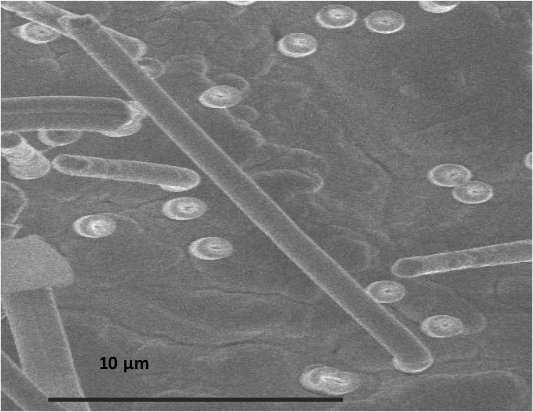
\includegraphics[height=0.35\textwidth]{PC}
			\hfill
			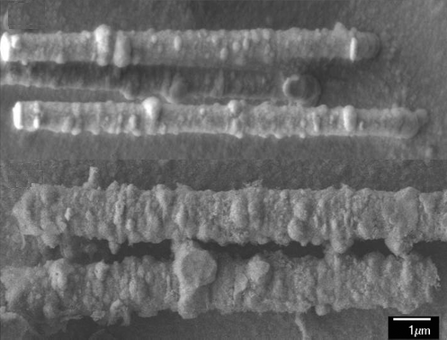
\includegraphics[height=0.35\textwidth]{PET}
			\hfill
			\caption{\textbf{Scanning electron microscope images of metal replica of track-etched PC (left) and PET (right) pores.} The pores were filled with metal and the polymer was completely etched a way, leaving a metal structure that is the inverse image of the pore. The metal was imaged in a scanning electron microscope. While the PC pores are nearly perfectly cylindrical in shape, the PET pores are characterized by rough inhomogenities across their entire surface, punctuated with large local bumps. The large bumps in the images of the metal replicas correspond to equally large cavitities in the PET pore.}
			\label{fig:PCPET}
		\end{figure}
		
		\begin{figure}
			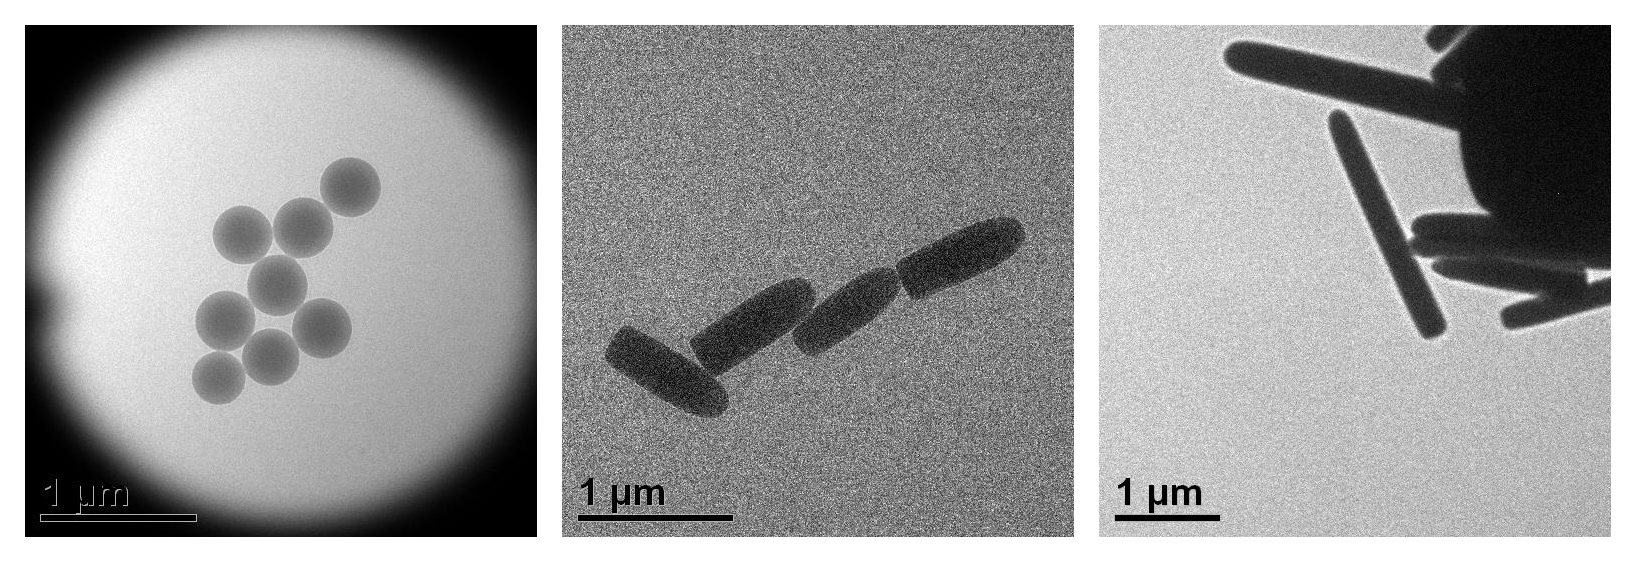
\includegraphics[width=1\textwidth]{particles}
			\caption{\textbf{Transmission electron microscope images of polystyrene beads and silica nanorods.} While the polystyrene beads are nearly perfectly spherical, the silica nanorods are approximately `bullet shaped'. For the purposes of this work, we approximated their shapes as ellipsoids in order to apply equation \ref{eq:dIellipsoid}.}
			\label{fig:particles}
		\end{figure}
		
		\begin{figure}
			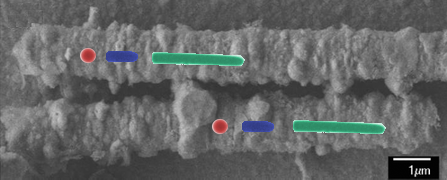
\includegraphics[width=\textwidth]{particles_real_size.png}
			\caption{\textbf{Images of particles alongside PET pores, to scale.} Notice that the spheres and rods are small enough to accurately map the interiors of the pores, since their length is comparable to or smaller than the length of the length scale of the irregularities in the pore. On the other hand, the long rods extend along many such irregularities at any given time, and hterefore will produce low-resolution maps of the pores' interiors.}
			\label{fig:particles_real_size}
		\end{figure}



	    
		In order to test the method described above for determining the lengths of particles, we performed resistive pulse experiments with single mesopores ranging from $800-\SI{1000}{nm}$ in diameter. The materials used were polyethylene terephthalate (PET), a polymer which is known to have highly irregularly shaped interiors when pores are prepared \textit{via} the track-etch technique, and polycarbonate (PC), another polymer but with no axial inhomogeneities. The PET pore will be used to test the length measurement protocol, while the PC pore will be used as a control pore. Figure \ref{fig:PCPET} shows images of both of these types of pores. For the particles, $\SI{280}{nm}$ and $\SI{410}{nm}$ in diameter polystyrene beads (`spheres') and rods of length $\SI{590}{nm}$, diameter $\SI{210}{nm}$ (`short rods') and $\SI{1920}{nm}$, diameter $\SI{240}{nm}$ (`long rods'). The particles are shown in figure \ref{fig:particles}, and a figure showing the relative sizes of the particles to the PET pores is shown in figure \ref{fig:particlespores}. Particles were suspended in $\SI{100}{mM}$ KCl solution with $0.5\%$ Tween 80, a surfactant which prevents particle aggregation. The solution was then injected into both sides of a conductivity cell, and a voltage was applied across the pore. The resulting ionic current was sampled at $\SI{10}{kHz}$ and recorded. The polystyrene spheres used had a larger $\zeta-\mathrm{potential}$ than the pore, and therefore they translocated through the pore electrophoretically. On the other hand, the rods had a lower magnitude $\zeta-\mathrm{potential}$ than the pore, and therefore travelled through the pore under electroosmotic convective forces.
		
	
	\section{Analysis \& Discussion}
	
	
		\begin{figure}
			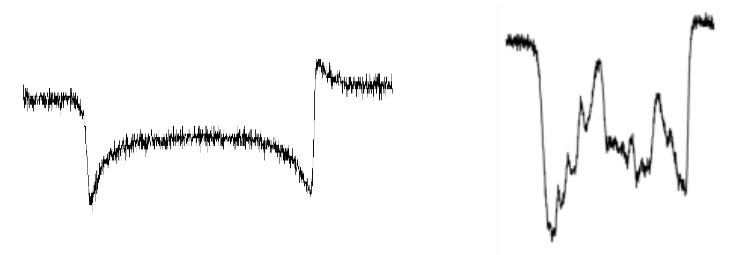
\includegraphics[width=0.5\textwidth]{PCPETevents}
			\caption{\textbf{Resistive pulse events through PC (left) and PET (right) pores.} As expected, the PET events are highly irregular and reflect the interior irregularities of the PET pore itself. On the other hand, the PC pores show no such irregularity. The events show that PC pores have large resistances at the beginning and end, reflecting the narrow, `pinched' diameters at the openings of the pores.}
			\label{fig:PCPETevents}
		\end{figure}

	
		\subsection{Anomalous resistive pulse amplitude for short rods}
			Events were extracted from the current time series and studied separately; figure \ref{fig:PCPETevents} shows two events, one from a PC pore and one from a PET pore that are representative of the translocations through each type of pore. In the initial analysis, we looked at the average $\Delta I/I_{p}$ of the beads and rods and compared with the theoretical predictions of Eqs. \ref{eq:dI} and \ref{eq:dIellipsoid}. 
			
			
			\begin{figure}
				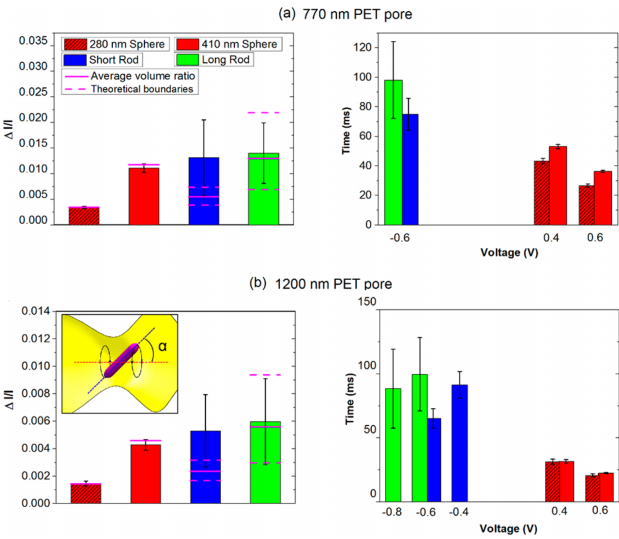
\includegraphics[width=\textwidth]{dIexp}
				\caption{\textbf{Resistive pulse amplitude average and standard deviation for the particles studied in two types of pores and their theoretical predictions (left), and event duration versus voltage plots (right).} The experimental predictions for the resistive pulse amplitudes are largely correct, except for the short rod events (blue box), which is off by at least a factor of two in both cases.}
				\label{fig:dIexp}
			\end{figure}

			
			Figure \ref{fig:dIexp} shows the results for two pores, one $\SI{770}{nm}$ and another $\SI{1200}{nm}$ in diameter. For the two spheres studied, the measured $\Delta I/I_{p}$ was very close to the theoretical prediction (Eq. \ref{eq:dI}). The theoretical predictions were also very close to the measured values for the long rods. However, for both pores the theoretical prediction of the resistive pulse amplitude $\Delta I/I_{p}$ is far off for the short rods: the data shows a nearly 100\% discrepancy, i.e.~ the measured $\Delta I/I_{p}$ is nearly twice its expected value. This significant of a discrepancy is highly unusual, and one of the goals in the paper was to determine its cause. The discrepancy is made even stranger by the fact that the short and long rods are made of silica, so any material contribution to the discrepancy e.g.~due to large $\zeta-\mathrm{potentials}$ is unlikely. Instead, we hypothesize that this discrepancy is due to their rotational dynamics. Equation \ref{eq:dIellipsoid} predicts that a prolate spheroid (like the rods) will have a larger $\Delta I/I_{p}$ when they are oriented with an off-axis component, but only considers static positioning. A very large rotational speed of the rods could couple to the measured $\Delta I/I_{p}$ amplitude in ways not captured by the equation, for instance by stirring the local solution in such a way that the local ion mobility---and hence conductivity---is reduced. Furthermore, this hypothesis is consistent with the non-observance of the increased $\Delta I/I_{p}$ for the long rods, since at their length of $\sim\SI{1920}{nm}$ they are too large to fully rotate in even the larger of the two pores ($\SI{1200}{nm}$ in diameter). In any case, the net result is a measured volume for these particles that is approximately $2\times$ larger than their actual volume, which was confirmed with a combination of transmission electron microscopy images and dynamic light scattering. 
			
			The question, however, is how such a large rotation could occur. The estimated rotational diffusion contribution of these rod particles is estimated as $\SI{13}{rad/s}$ and $\SI{0.8}{rad/s}$ for the short and long rods, respectively \cite{Tirado1980}. The fluid flow in the channel is due to electroosmosis, and due to continuity constraints on the fluid motion, variations in the local average pore radius could induce axial variations in the fluid flow speed. These axial variations could torque the rod. However, as a more likely culprit for the source of the torque, we considered the effect of the electric field on the particle. Rough undulations in the pore create axial variations in the electric field and such variations could also lead to a net torque on the particle that causes rotation. In order to estimate the potential magnitude of the rotational velocities of the rods, we considered a simple model where the pore's diameter discontinuously changes from $\SI{1000}{nm}$ to $\SI{1100}{nm}$, a reasonable approximation for the geometries present in our system based on the images of the pores (see Fig. \ref{fig:PCPET}). Under this model, we calculate the electric field amplitude to differ by a factor of $1.2$ between the two regions. Using the rotational diffusion coefficient of the rods and integrating the electric field differences along the length of the particle, we calculate the angular rotation rate $\omega$ to be $\omega\sim10^{4}$ rad/s. Due to the preceding arguments, it is clear that the largest contribution to the rotation of the rods is from the electric forces. We believe that such a large rotation could make the rods behave as if they were effectively much larger particles.
		
		\subsection{Length measurement protocol test}
		
		
			\begin{figure}
				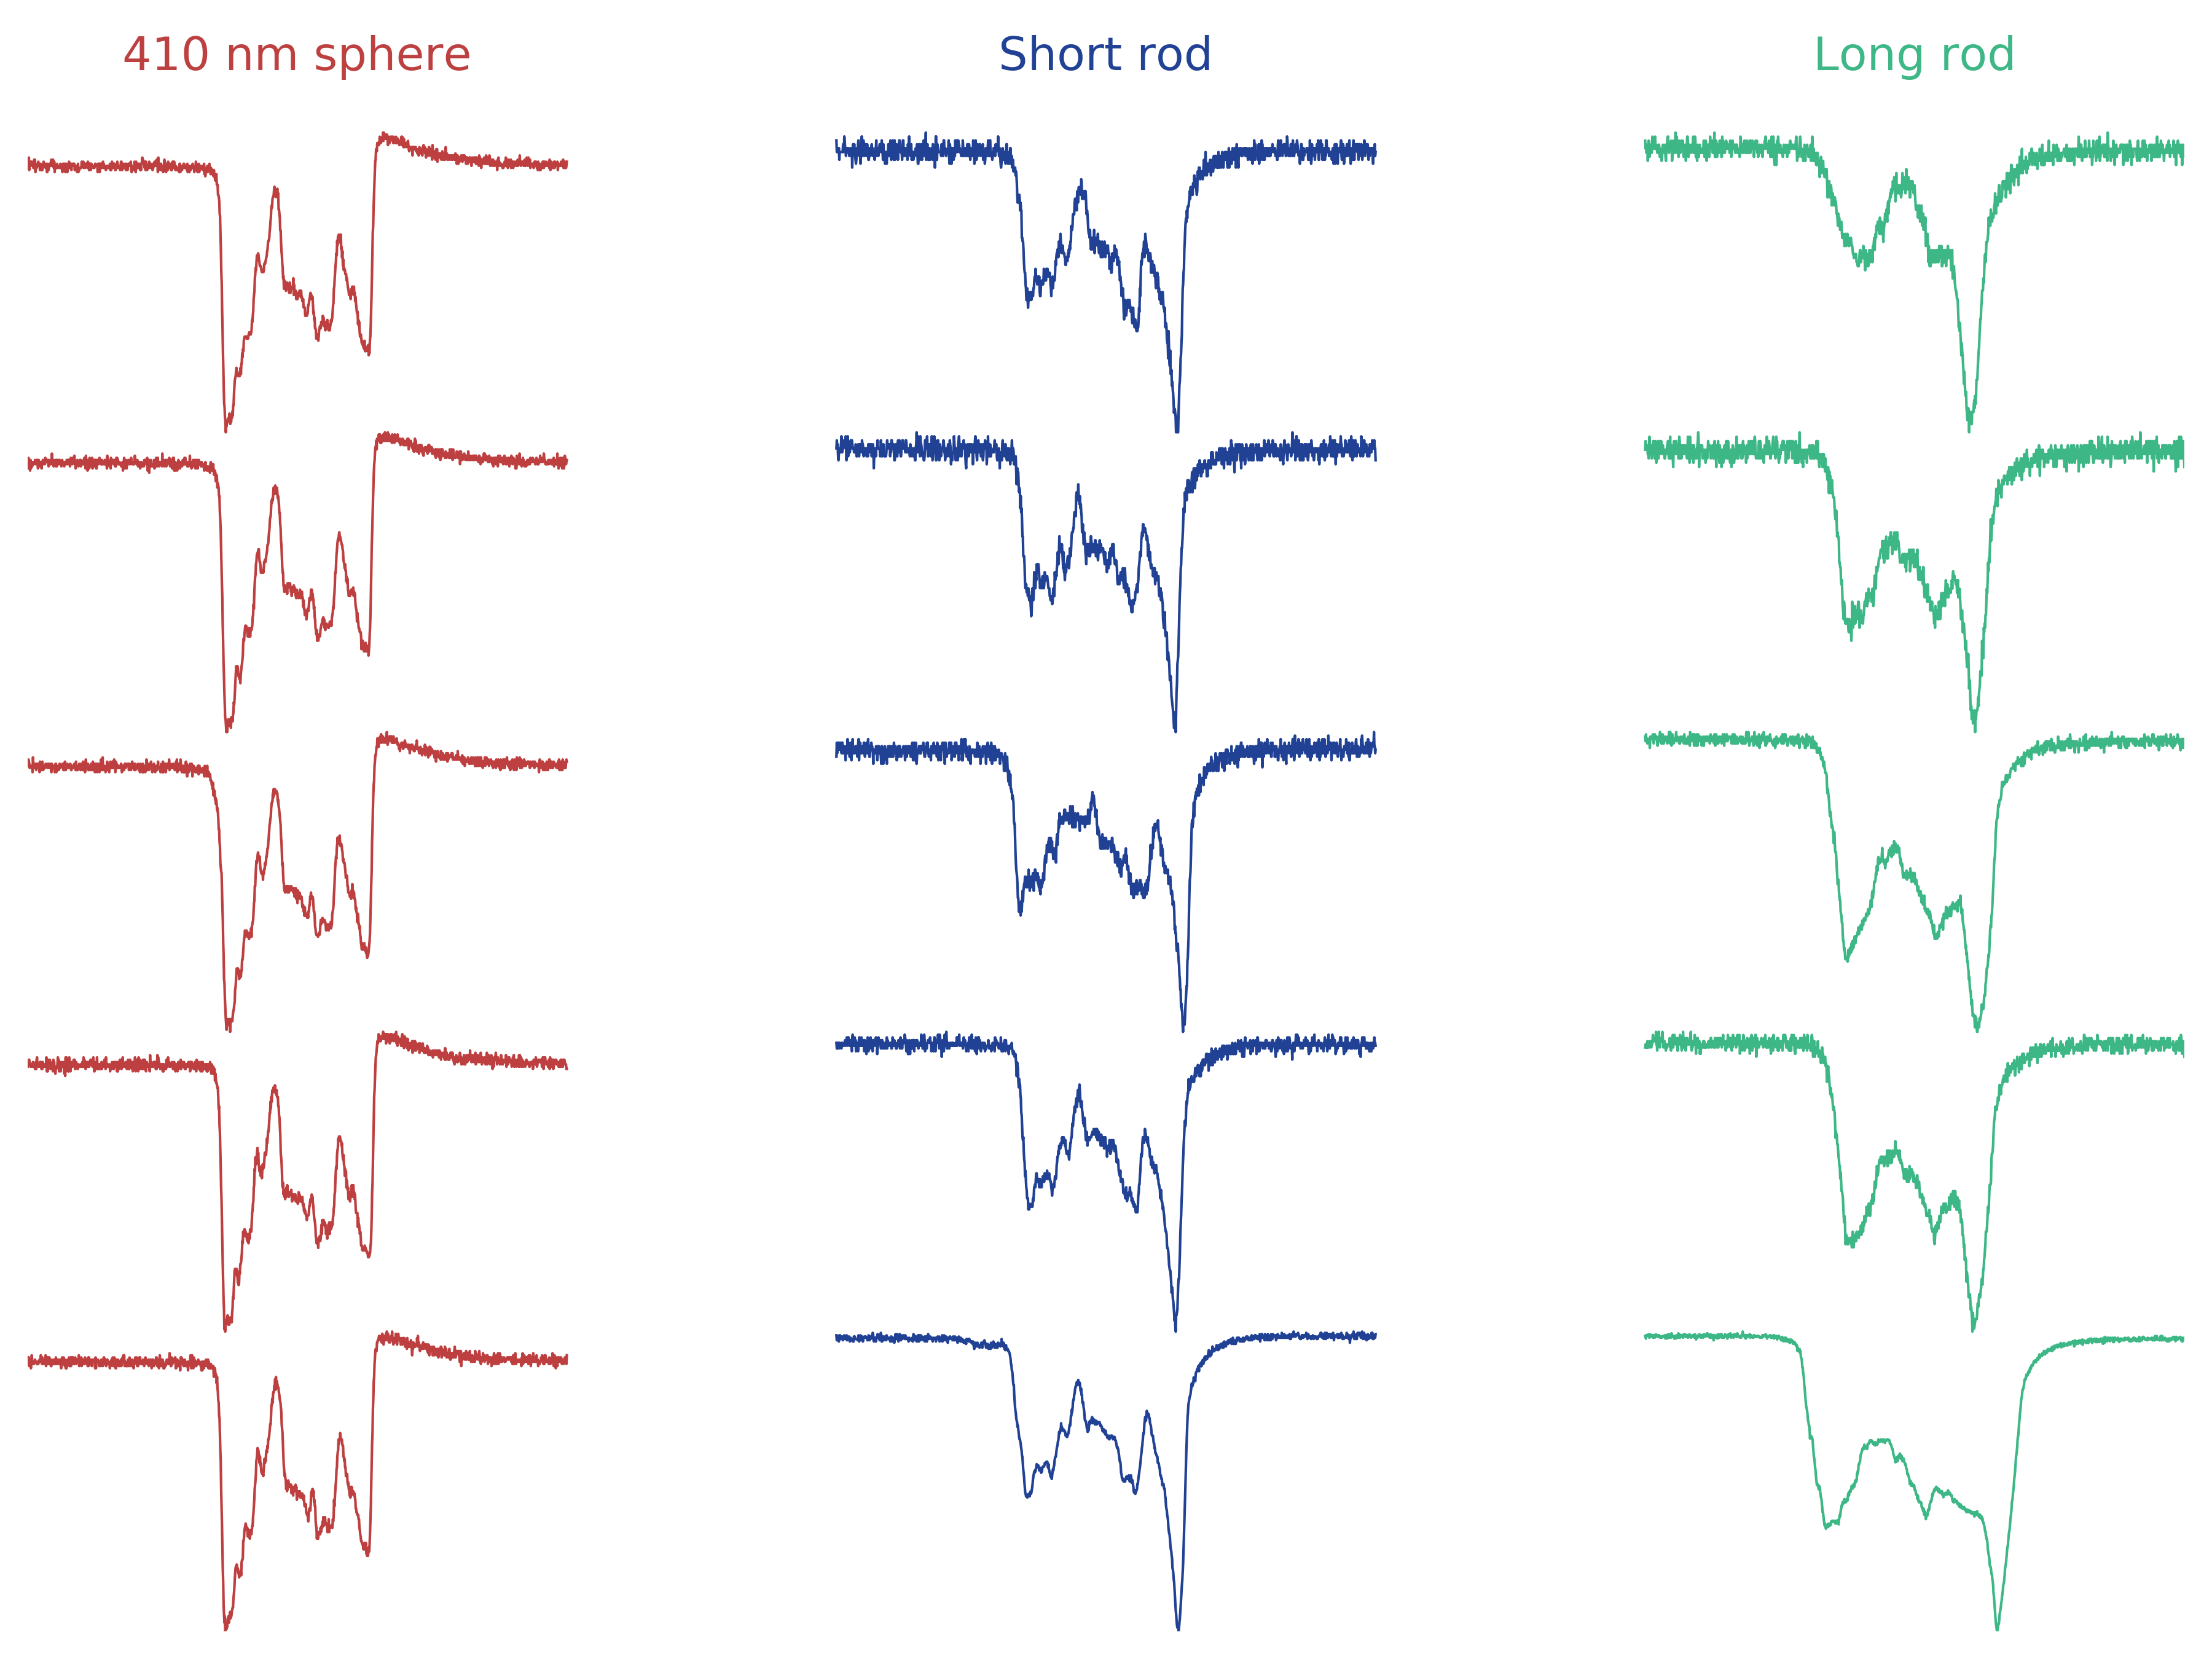
\includegraphics[width=\textwidth]{PET21_raw.png}
				\caption{\textbf{Resistive pulse events for polystyrene spheres, short rods, and long rods through a particular PET pore.} The pulses indicate that the resistive pulse process is repeatable, as only small variations exist from signal to signal. While the signals of the spheres and rods are similar, in agreement with the model presented for how they accurately resolve the interior features of the channel, the signals of the long rods are quite different. Each of the long rod signals resembles the signals of the spheres and short rods, but with less resolution.}
				\label{fig:PET21_raw}
			\end{figure}

		
			Next, we return to the idea of using the PET pore signals to measure the lengths of unknown particles. Figure \ref{fig:PET21_raw} shows sample events of the three types of particles used in this study.
		
			\begin{figure}
				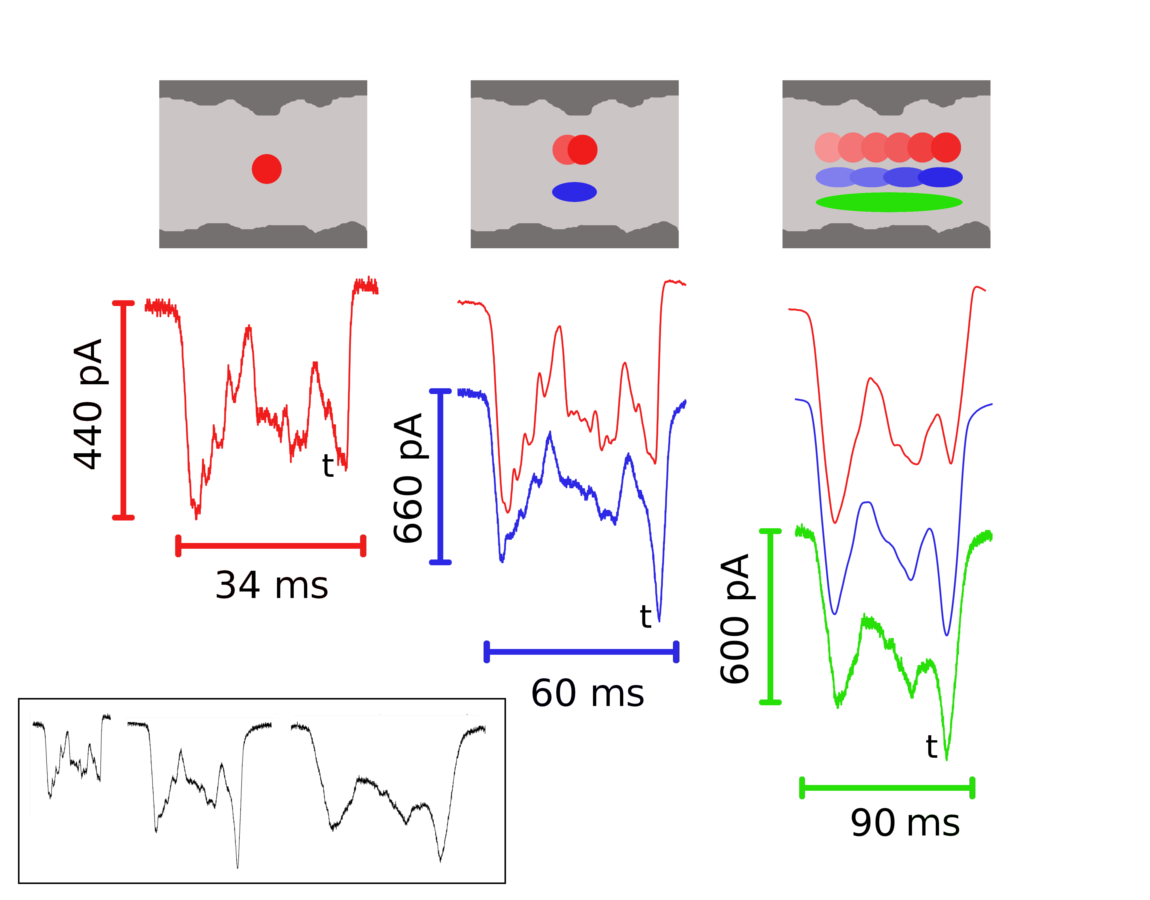
\includegraphics[width=.5\textwidth]{PET21_qualitative}
				\caption{\textbf{Resistive pulse events of a $\SI{410}{nm}$ diameter sphere (red), and $\SI{590}{nm}$ (blue) and $\SI{1920}{nm}$ (green) in length rods.} The top row shows a cartoon scheme of the pore with the particles inside its interior. The bottom resistive pulse event in each column corresponds to the raw recorded data; events above this are smoothed \textit{via} the moving average transformation. The bottom left figure shows the raw events on the same scale.}
				\label{fig:PET21_qualitative}
			\end{figure}

			In order to demonstrate the qualitative differences between the signals of the long rods and the signals of the spheres and short rods, we plot three representative samples together in Fig. \ref{fig:PET21_qualitative}. The top signal of each column in the figure shows the raw signal of each of the particles. We plot the signals that have been transformed \textit{via} the moving average process below these raw signals. The time over which the moving average was calculated corresponded to the duration in time over which the particle travelled a distance equal to the length of the longer particle with which it is being compared. We determined the average velocity of a particle from the total translocation distance (the known length of the pore, $L'=L-D$) and the translocation duration measured from the RP signal, $\Delta T$. The velocity is then $v=L'/\Delta t$. The moving average window then has length (in time) of $\Delta t=v/l$, which corresponds to a window of $N=f\times\Delta t$ data points in length. In the central column, the transformed sphere and short rod bear similarity, but this is unsurprising due to the fact that their resistive pulses are high resolution mappings of the channel. On the other hand, in the third column we show the transformed signals of the sphere's signal and the short rod's signal under the long rod's raw signal. Notice that the moving average transformation, for both the sphere and the short rod, has produced a signal that is qualitatively very similar to the long rod. In particular, the sub-minima and maxima in each of the raw signals of the short particles have disappeared, leaving only the larger scale features in the signals. Without making any quantitative arguments, we are able to conclude that the particle corresponding to the green event is longer than the particle corresponding to the red and blue events event. 
			
			In order to test the quantitative algorithm for particle length determination, we used the short rods as the `tracer particle'. In principle we could use the signal of the sphere, but while their moving average signal is qualitatively similar to the long rod's signal, it still differs in significant ways. In particular, the initial and final minima have drastically different amplitudes. This effect is due to entrance/exit effects related to increased sourcing of ions due to the charge of the particle, and is therefore expected \cite{Menestrina2014}. 
			
			
			\begin{figure}
				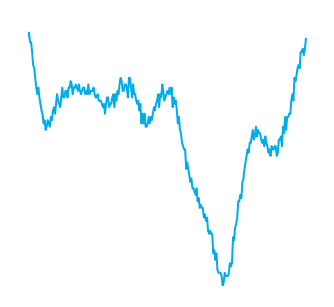
\includegraphics[width=0.5\textwidth]{longevent.png}
				\caption{\textbf{Resistive pulse signal of a single long rod passing through a PET pore.} The variation in the amplitude of the current signals that the pore has an inhomogeneous interior shape.}
				\label{fig:longevent}
			\end{figure}

			
			\begin{figure}
				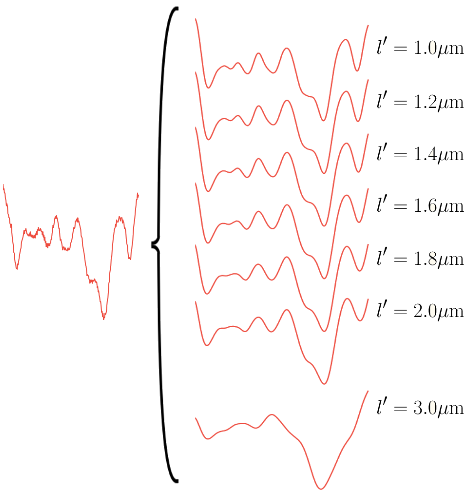
\includegraphics[width=0.5\textwidth]{experimentaldtwfits.png}
				\caption{\textbf{Resistive pulse signal of a single short rod passing through a PET pore alongside many instances of the moving average transformation performed on the signal for different length intervals.} As the length interval is increased, the finer structure of the resistive pulse signal is smoothed over. For the greatest length measured, many of the features prominent in the raw signal have disappeared..}
				\label{fig:experimentaldtwfits}
			\end{figure}
			
			
			\begin{figure}
				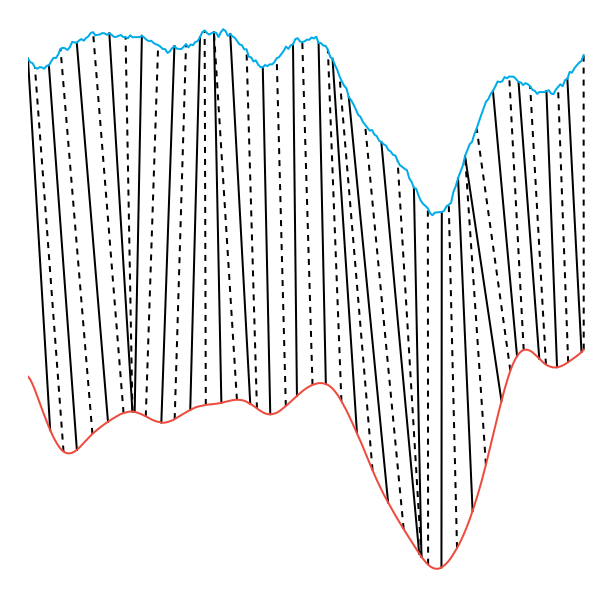
\includegraphics[width=0.5\textwidth]{experimentaldtwfit.png}
				\caption{\textbf{Raw resistive pulse signal of a single long rod matched with the signal of a short rod that has been transformed via the moving average process.} The aligned points were determined by the dynamic time warping algorithm, and the particular transformation shown was the one that minimized the difference between the two signals, also determined by the dynamic time warping algorithm.}
				\label{fig:experimentaldtwfit}
			\end{figure}
			
			
			In order to measure the lengths of the long rods, we performed the dynamic time warping technique described in the preceding section. Figure \ref{fig:experimentaldtwfits} shows a shorter rod particle averaged over many different length intervals. As the short rod is averaged over a greater length interval, it continuously transforms into a shape that bears a stronger resemblance to the signal of the long rods. Of all the fits calculated in Fig. \ref{fig:experimentaldtwfits}, the correct length is determined by the fit with the smallest cost as determined by dynamic time warping. An example resistive pulse signal of a long rod and a shorter rod that has been transformed \textit{via} the moving average equation is shown in Fig. \ref{fig:experimentaldtwfit}. Finally, after performing the moving average and dynamic time warping minimization approach described above, we were able to determine the expected lengths of the long rods according to this algorithm. Figure \ref{fig:dtwfit} shows a plot of histograms of the lengths as determined by this approach, alongside a Gaussian fit to the histogram, and a Gaussian distribution that shows the actual distribution of hte lengths of the long particles as determined by electron microscopy images. The figure reveals that, in this case, the dynamic time warping algorithm is able to successfully recover the real distribution of the known lengths relatively accurately.
			
			
			\begin{figure}
				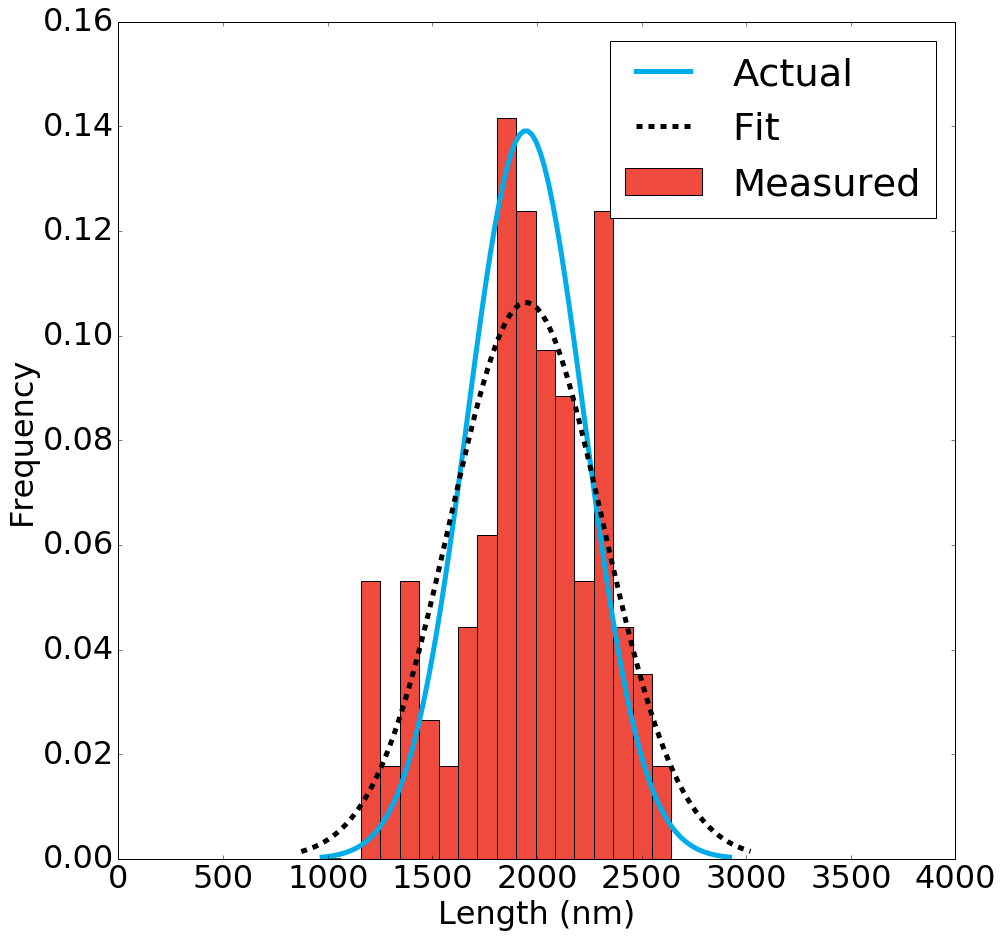
\includegraphics[width=0.5\textwidth]{dtwfit.png}
				\caption{\textbf{Histogram of particle length as determined by dynamic time warping along with the actual distribution of sizes determined by electron microscopy imaging.} A normal distribution is fit to the histogram of particle lengths as determined by dynamic time warping and shown to be in good agreement with the expected distribution.}
				\label{fig:dtwfit}
			\end{figure}
		
	\section{Conclusions}
		In summary, we presented resistive pulse experiments performed with spherical and non-spherical particles in two types of pores, those with smooth interiors (PC) and rough interiors (PET). We devised a protocol for measuring the lengths of long particles by taking advantage of the rough interiors of PET pores, which reflect in the measured resistive pulse signals of all the particles. Longer particles displace a greater distance along the pore's length, and therefore their signals are a more smoothed version of the signals of shorter particles. This smoothing attribute can be recovered by taking the moving averages of shorter particles. By performing moving averages for many different particle lengths and measuring the similarity between the raw signal of the long particles with each of the transformed signals of the shorter particles, we were able to determine the length distribution of the long particles used in experiments. Dynamic time warping was used as a means of effectively comparing the similarity of the signals of the two particles. While the general premise of the `smoothing' of the resistive pulse signals by long particles compared to short particles is convincingly established, more research must be performed on the hybrid moving average-dynamic time warping method. The protocol was only tested for a small number of pores and only two types of particles, short and long rods. In the future, an ideal experiment could be performed with short rods of known length, and rods of various unknown lengths. The experiments and analysis would be performed in a blind fashion, and only after the analysis is complete would the true length distribution of the long rods be revealed. If the length measurement protocol survives this blind study, it would prove to be a very effective means of determining the lengths of particles.
		
		Additionally, an unrelated phenomena was discovered where short, aspherical particles created far greater (up to 2x) resistive pulse amplitudes than predicted by the well-established classical equations. The exact reason for this effect is still unknown, however we laid out arguments that explain rotational dynamics as a likely culprit. We reasoned from our studies that an extremely rapid rate of rotation could effectively increase the radius of the particle, possibly by disturbing the local solution and decreasings its conductivity. Such rotations would not be possible for the longer rods due to their prohibitively long lengths compared to the diameter of the pore. However, more investigation must be performed in order to convincingly show that not only do short rod like objects deviate strongly from the classical equations, but also that rotational dynamics is the culprit. Additional experiments must be performed with a larger variety of short rods to show that the effect is general and not limited to the rods used in this study. Furthermore, experiments could be designed in such a way as to retard the rods' rotations, perhaps by using smaller pores or solution with an increased viscosity.

	
	
		
		
		
	

	




%%% Local Variables: ***
%%% mode: latex ***
%%% TeX-master: "thesis.tex" ***
%%% End: ***
